\section{Deployment Contracts and Claim Scope}
\label{sec:contracts}

\subsection{Prediction task and label eligibility}
Let a temporal fraud task be
\(
D=(\mathcal{I},X,t,y,G_0,U),
\)
where $\mathcal{I}$ indexes candidate predictions, $X$ contains observed attributes, $t_i$ is event time, $G_0$ is the source relational record, and $U$ identifies the prediction unit. The three units studied here are a transaction node, an account node, and a transaction edge. Metrics are comparable within a unit and contract; we do not pool their values into a cross-task leaderboard.

The repository label convention for Elliptic and DGraphFin is
\(
y_i\in\{0,1,2\},
\)
with $0$ denoting unknown or ineligible, $1$ fraud, and $2$ normal. Supervision is defined only on
\begin{equation}
    m_i=\mathbf{1}[y_i\ne 0], \qquad
    z_i=\mathbf{1}[y_i=1] \quad \text{for } m_i=1 .
    \label{eq:eligibility}
\end{equation}
Thus unknown labels never enter a train, validation, or test mask. IBM AML-Data is materialized directly as the binary edge label $z_i=\texttt{is\_laundering}_i$ and has no unknown class in the evaluated task. A fitted model produces a score $s_i\in\mathbb{R}$ for each eligible evaluation unit.

\subsection{Deployment contract}
A deployment contract is the six-tuple
\begin{equation}
    \Pi=(\mathcal{T},\mathcal{V},\mathcal{C},\mathcal{S},\mathcal{B},\mathcal{R}).
    \label{eq:deployment-contract}
\end{equation}
Its coordinates are recorded separately and are non-substitutable: holding one
fixed does not make a change in another scientifically ignorable. They need not
be statistically or causally independent.
\begin{itemize}
    \item $\mathcal{T}$ fixes temporal order, train/validation/test intervals, and prediction horizon.
    \item $\mathcal{V}$ states which nodes and edges are visible when features are constructed, the model is fitted, and predictions are made. Label visibility is specified separately.
    \item $\mathcal{C}$ maps the source record $G_0$ to the evaluated graph and attributes. It includes the prediction unit, direction, edge features, degree limits, and historical window.
    \item $\mathcal{S}$ records the validation data, model-selection metric, stopping rule, and threshold-selection policy.
    \item $\mathcal{B}$ defines the decision surface: a threshold, review capacity $K$, selective coverage, or explicit error costs.
    \item $\mathcal{R}$ declares the hardware and software envelope, memory and disk guards, runtime measurement, and failure semantics.
\end{itemize}
Two contracts can share a chronological split while differing in graph access, or share a graph while answering different review-budget questions. Comparisons across contracts must name the components that changed.

Figure~\ref{fig:deployment-contract} summarizes the information flow. The contract fixes the scientific scope before a run becomes evidence; the support test then checks whether the requested claim is covered.

\begin{figure*}[t]
    \centering
    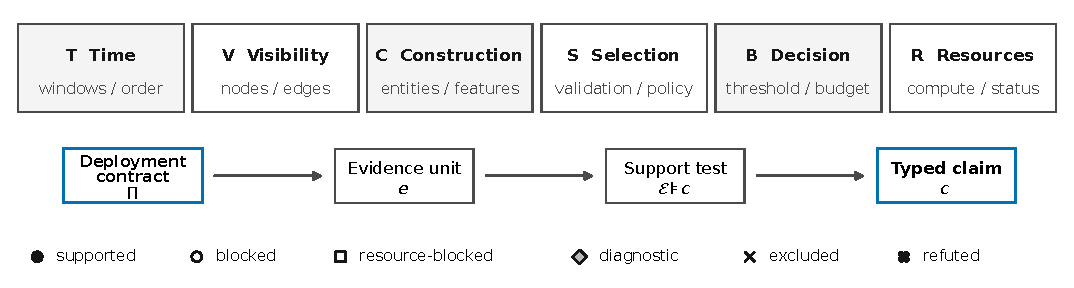
\includegraphics[width=\textwidth]{figures/fig01_deployment_contract.pdf}
    \caption{FraudShiftBench information flow. Six non-substitutable coordinates define a deployment contract. A run becomes a typed evidence unit, and the support test admits only claims covered by its scope, predictions, uncertainty, integrity, and resource state. Blocked evidence has no implied performance value.}
    \label{fig:deployment-contract}
\end{figure*}

\subsection{Evidence units and typed claims}
A result file alone is not the evidence object. We define
\begin{equation}
 e=(D,\nu,U,\Pi,C_G,M,H,\Sigma,Q,P,R_e,Z),
 \label{eq:evidence-unit}
\end{equation}
where $\nu$ is the dataset variant, $C_G$ is the concrete graph materialization, $M$ and $H$ identify the method and hyperparameters, $\Sigma$ is the seed set, and $Q$ is the metric set. $P$ points to prediction-level outputs, $R_e$ records measured resource outcome, and $Z$ contains provenance and integrity state. $C_G$ is retained even though construction is part of $\Pi$: the contract states the scientific choice, while $C_G$ identifies its realized artifact and parameters.

A claim is also typed:
\begin{equation}
 c=(\Omega,q,\Delta,\mu,d,u,\iota).
 \label{eq:typed-claim}
\end{equation}
Here $\Omega$ is the dataset/model/protocol scope, $q$ is a quantifier, $\Delta$ names the comparison, $\mu$ is the metric, $d$ is the asserted direction or ordering, $u$ specifies uncertainty and multiplicity requirements, and $\iota$ gives the deployment interpretation. For example, ``GraphSAGE loses AUPRC under isolated access on Elliptic'' and ``graphs are harmful'' differ in both scope and quantifier even if they cite the same cell.

For a set of evidence units $\mathcal{E}$, we write $\mathcal{E}\models c$ only if all of the following hold: (i) every cell required by $\Omega$ and $q$ is present under a compatible contract; (ii) $Z$ passes the declared schema, provenance, and construct checks; (iii) $P$ is present whenever the claim requires prediction-derived metrics or reanalysis; (iv) the specified seeds and paired keys are complete; (v) the test, effect, interval, and multiplicity procedure in $u$ can be executed; (vi) no requested predictive comparison crosses a resource-blocked cell; and (vii) the observed predicate $d$ is true. The benchmark returns \emph{supported}, \emph{blocked}, \emph{resource-blocked}, \emph{diagnostic-only}, \emph{excluded}, or \emph{refuted in scope}. Blocked denotes inadequate evidence. Refuted denotes complete evidence that contradicts the predicate.

\subsection{Useful consequences}
The relation has four immediate properties.

\emph{Scope monotonicity.} If $c'$ widens the scope or quantifier of $c$, its required cell set contains that of $c$. Evidence sufficient for the narrower claim is not thereby sufficient for $c'$.

\emph{Evidence restriction.} Removing a required seed, prediction manifest, or cell cannot upgrade an unsupported claim. This follows directly because each is a conjunct in the support test.

\emph{Protocol non-equivalence.} Evidence under $\Pi_1$ may support a claim stated for $\Pi_2$ only when the components relevant to that claim coincide. Equal numerical values do not establish that two estimands are interchangeable.

\emph{Rank and resource separation.} For scores without a change in tie order, a strictly increasing transform preserves the order used by AUROC and AUPRC, although a fixed threshold can yield different decisions \cite{guo2017calibration}. A resource-blocked cell has no predictive score and therefore has no position in either ranking.

The validator implements these requirements over immutable inventory records. Its role is deliberately limited: it can detect an unsupported scope expansion or an absent prediction manifest, but it cannot establish construct validity or causal explanation by itself.
